\chapter{Lecture}\label{part2:lec12}
\markboth{\thechapter. Lecture}{\thechapter. Lecture}

We\pageoriginale now come to a rather important topic, the
transformation of $\mathscr{V}$-functions. So far we have been looking
upon $\mathscr{V}_\alpha (\mathscr{V}/ \tau)$ as a function of
$\mathscr{V}$ only; hereafter we shall be interfering with the
`period' $\tau$ also. We want to study how $\mathscr{V}_\alpha
(\mathscr{V}/ \tau)$ changes when $\mathscr{V}$ is replaced by
$\mathscr{V}+ 1/\tau$. For this it is enough if we replace
$\mathscr{V}$ by $\mathscr{V} \tau = \omega$ and see how the function
behaves when $\omega$ is changed to $\omega+1$. This would amount to
turning the whole plane around in the positive sense about the origin
through arg $\tau$. We take $\mathscr{V}_1$, because it is easier to
handle, since the zeros become the periods too. Consider
$$
f(\mathscr{V}) = \mathscr{V}_1 (\mathscr{V} \tau/\tau)
$$

Then 
\begin{align*}
  f(\mathscr{V}+1) & = \mathscr{V}_1 ((\mathscr{V}+1)\tau / \tau)\\
  & = \mathscr{V}_1 (\mathscr{V} \tau + \tau/\tau)\\
  & = - e^{-\pi i \tau} e^{-2 \pi i \mathscr{V} \tau} \mathscr{V}_1
  (\mathscr{V} \tau/ \tau)\\
  & = e^{- \pi i \tau} e^{- 2 \pi i \mathscr{V} \tau} f(\mathscr{V})
\end{align*}

$\tau$ Similarly consider $f(\mathscr{V}- 1/\tau)$ (We choose to take
$- \frac{1}{\tau}$ rather than $\frac{1}{\tau}$ since we want the
imaginary part of the parameter to be positive:
\begin{align*}
  \im \frac{1}{\tau} & = \im \frac{\bar{\tau}}{\tau \bar{\tau}} < 0
  ~\text{and so}~ \im  - \frac{1}{\tau} > 0)\\
  f(\nu - \frac{1}{\tau}) & = \mathscr{V}_1 ((\nu - \frac{1}{\tau})
  \tau/\tau)\\
  & = \mathscr{V}_1 (\mathscr{V} \tau - 1/ \tau)\\
  & = - \mathscr{V}_1 (\mathscr{V} \tau/ \tau)\\
  & =- f(\mathscr{V})
\end{align*}
So\pageoriginale $f$ is a sort of $\mathscr{V}$-function which picks up simple
factors for the `periods' 1 and $- \frac{1}{\tau}$. $f(\mathscr{V})$
has clearly zeros at 0 and $\tau' =-\frac{1}{\tau}$, or generally at
$\mathscr{V} = m_1 + m_2 \tau'$; $m_1, m_2$ integers, which is a
point-lattice similar to the old one turned around. 

Similarly let us define
\begin{align*}
  g(\mathscr{V}) & = \mathscr{V}_1 (\mathscr{V}/ \tau') =
  \mathscr{V}_1 \left(\mathscr{V}/- \frac{1}{\tau}\right)\\
  g(\mathscr{V}+1) & = \mathscr{V}_1 (\mathscr{V}+ 1/\tau')\\
  & = - \mathscr{V}_1 (\mathscr{V}/ \tau')\\
  & = - g(\mathscr{V})\\
  g\left(\mathscr{V}- \frac{1}{\tau}\right) & = g(\mathscr{V}+ \tau')\\
  & = \mathscr{V}_1 (\mathscr{V}+ \tau'/\tau')\\
  & = - e^{-\pi i \tau'} e^{- 2 \pi i \mathscr{V}} \mathscr{V}_1
  (\mathscr{V}/ \tau')\\
  & =- e^{\pi i/\tau} e^{- 2 \pi i \mathscr{V}} g(\mathscr{V})
\end{align*}

Let\pageoriginale us form the quotient:
\begin{align*}
  \Phi (\mathscr{V}) & = \frac{f(\mathscr{V})}{g(\mathscr{V})}\\
  \phi (\mathscr{V}+1) & = \frac{f(\mathscr{V}+1)}{g(\mathscr{V}+1)}\\
  & = -e^{-\pi i \tau} e^{-2\pi i \mathscr{V} \tau} \phi
  (\mathscr{V})\\
  \Phi \left(\mathscr{V}- \frac{1}{\tau}\right) & = \frac{f(\mathscr{V}+
    \tau')}{g(\mathscr{V}+ \tau')}\\
  & = \frac{f(\mathscr{V})}{e^{\pi i/\tau} e^{- 2 \pi i \mathscr{V}}
    g(\mathscr{V})}\\
  & = e^{- \pi i / \tau} e^{2 \pi i \mathscr{V}} \Phi (\mathscr{V}) 
\end{align*}

$\Phi$ takes on simple factors in both cases of this peculiar sort
that we can eliminate them both at one stroke. We write
\begin{align*}
  e^{- \pi i \tau (2 \mathscr{V}+1)} \Phi (\mathscr{V}) & = \Phi
  (\mathscr{V}+1),\\
  e^{\pi i (2 \mathscr{V}-1/\tau)} \Phi (\mathscr{V}) & = \Phi (\mathscr{V}-1/\tau)
\end{align*}

Let us try the following trick. Let us supplement $\Phi (\mathscr{V})$
by an outside function $h(\mathscr{V})$ so that the combined function
$\Phi(\mathscr{V})$ is totally doubly periodic. Write 
$$
\Psi (\mathscr{V}) = \Phi (\mathscr{V}) e^{h(\mathscr{V})}
$$ 

We\pageoriginale want to choose $h(\mathscr{V})$ in such a manner
that
$$
\Psi (\mathscr{V}+1) = \Psi (\mathscr{V}+ \tau')= \Psi (\mathscr{V})
$$

This implies two equations:
\begin{align*}
  e^{- \pi i \tau (2 \mathscr{V}+1)} e^{h(\mathscr{V}+1)-
    h(\mathscr{V})} & = 1\\
  e^{\pi i (2 \mathscr{V}-1\tau)} e^{h(\mathscr{V}- 1/\tau)-
    h(\mathscr{V})}& = 1;
\end{align*}
or
\begin{align*}
  h(\mathscr{V}+1) - h(\mathscr{V}) & = \pi i \tau (2 \mathscr{V}+1) +
  2 \pi i m\\
  h(\mathscr{V}+ \tau'- h(\mathscr{V}) & = - \pi i (2 \mathscr{V}+
  \tau') + 2 \pi i m'.
\end{align*}

We can solve both at one stroke. Since on the right side we have a
linear function of $\mathscr{V}$ in both cases, a quadratic polynomial
will do what we want.
$$
(\mathscr{V}+ \delta)^2- \mathscr{V}^2 = 2 \mathscr{V}\delta +
\delta^2 = \delta (2 \mathscr{V}+ \delta),
$$
and taking $h(\mathscr{V})= \pi i \tau \mathscr{V}^2$,
\begin{gather*}
  h (\mathscr{V}+1)- h(\mathscr{V})= \pi i \tau (2 \mathscr{V}+1)\\
  h(\mathscr{V}+ \tau') - h(\mathscr{V}) = \pi i \tau \tau'
  (\mathscr{V}+ \tau') =- \pi i (2 \mathscr{V}+ \tau'),
\end{gather*}
so that both the equations are satisfied. Putting it in, we have
$$
\Psi (\mathscr{V}) = e^{\pi i \tau \mathscr{V}^2}
\frac{\mathscr{V}_1(\mathscr{V} \tau / \tau)}{\mathscr{V}_1
  \left(\mathscr{V}/ -\frac{1}{\tau}\right)}
$$

This\pageoriginale has the property that
$$
\psi (\mathscr{V} +1)= \psi (\mathscr{V} + \tau)= \psi (\mathscr{V}) 
$$

So we have double periodicity. This function is also
an entire function because the numerator and denominator have the same
simple zeros. So this is a pole-free function and hence a constant
$C$, $C$ a constant with respect to the variable $\mathscr{V}$, but
may be a function of the parameter $\tau, C= C(\tau)$. We thus have 

I. 
$$
e^{\pi i \tau \mathscr{V}^2} \mathscr{V}_1 (\mathscr{V} \tau/ \tau) =
C(\tau) \mathscr{V}_1 \left(\mathscr{V}/-\frac{1}{\tau}\right) 
$$ 

What we need now are the corresponding formulas for the other
functions. Replacing $\mathscr{V}$ by $\mathscr{V}+ \frac{1}{2}$, 
$$
\displaylines{\hfill e^{\pi i \tau (\mathscr{V} + \frac{1}{2})^2}
    \mathscr{V}_1 \left(\left(\mathscr{V}+ \frac{1}{2}\right)
    \tau/\tau\right) = C(\tau) \mathscr{V}_1 \left(\mathscr{V}+ \frac{1}{2}
    \Big/- \frac{1}{\tau}\right),\hfill \cr
    \text{or} \hfill e^{\pi i \tau (\mathscr{V}^2 + \mathscr{V}+ 1/4)}
    i e^{-\pi i \tau/4} e^{- \pi i \mathscr{V} \tau} \mathscr{V}_4
    (\mathscr{V} \tau/ \tau) = C(\tau) \mathscr{V}_2 \left(\mathscr{V}/-
    \frac{1}{\tau}\right)\hfill }  
$$

We notices here that two different $\mathscr{V}$-functions are
related. This gives 

II. 
$$
i e^{\pi i \tau \mathscr{V}^2} \mathscr{V}_4 (\mathscr{V} \tau/ \tau)
= C(\tau) \mathscr{V}_2 \left(\mathscr{V}/ - \frac{1}{\tau}\right). 
$$

Replacing in I $\mathscr{V}$ by $\mathscr{V}+ \tau'/2= \mathscr{V}-
1/(2\tau)$, we get 

III. 
$$
i e^{\pi i \tau \mathscr{V}^2} \mathscr{V}_2 (\mathscr{V} \tau/\tau)=
C(\tau) \mathscr{V}_4 \left(\mathscr{V}/-\frac{1}{\tau}\right)
$$

Finally putting $\mathscr{V}+ \frac{1}{2}$ for $\mathscr{V}$ In, III,

IV. 
$$
ie^{\pi i \tau \mathscr{V}^2} \mathscr{V}_3 (\mathscr{V} \tau / \tau)
= C(\tau)\mathscr{V}_3 \left(\mathscr{V}/ - \frac{1}{\tau} \right)
$$

The\pageoriginale way the functions change over in I-IV is quite plausible. For
consider the location of the zeros. 

\medskip
\noindent
\begin{minipage}{3cm}
When we take the parallelogram and
turn it around what was originally a zero for  $\mathscr{V}_4$ becomes
one for $\mathscr{V}_2$ and vice versa; and what used to be in the
middle, the zero of $\mathscr{V}_3$, Remains in the middle. So the
formulae are plausible in structure. 
\end{minipage}
\begin{minipage}{7cm}
\begin{figure}[H]
  \centering{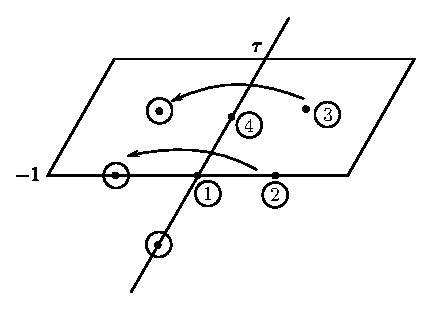
\includegraphics{vol2-figures/fig2.16.eps}}
\end{figure}
\end{minipage}

The most important thing now is, what is $C(\tau)$? To evaluate
$C(\tau)$ let us differentiate $I$ and put $\mathscr{V}=0$. We have

V.
$$
\tau \mathscr{V}^1_1(0 / \tau) = C(\tau) \mathscr{V}_1^1 \left(0 /
-\frac{1}{\tau} \right)
$$

From II, III, and IV, putting $\mathscr{V}=0$,
\begin{align*}
  i \mathscr{V}_4 (0/ \tau) & = C(\tau) \mathscr{V}_2 \left(0/ -
  \frac{1}{\tau}\right) \\
  i \mathscr{V}_2 (0/ \tau) & = C(\tau) \mathscr{V}_4 \left(0/ -
  \frac{1}{\tau}\right)\\ 
  i \mathscr{V}_3 (0/ \tau) & = C(\tau) \mathscr{V}_3 \left(0/ -
  \frac{1}{\tau}\right) 
\end{align*}

Multiplying these together and recalling that $\pi  \mathscr{V}_1'=
\mathscr{V}_2 \mathscr{V}_3 \mathscr{V}_4$, we obtain

VI.
$$
-i \mathscr{V}_1^1(0/ \tau) = (C(\tau))^3 \mathscr{V}_1' \left(0/
-\frac{1}{\tau}\right). 
$$

Dividing\pageoriginale by VI, by V, 
$$
\displaylines{\hfill \frac{1}{i \tau} = C^2 (\tau),\hfill \cr
  \text{or} \hfill C(\tau) = \pm \sqrt{\frac{1}{i \tau}} \hfill }
$$

In II, III, IV, it is $\frac{C(\tau)}{i}$ that appears; so let us
write this is 
$$
\frac{C(\tau)}{i} = \pm \frac{1}{i} \sqrt{\frac{1}{i \tau}} = \pm
\sqrt{\frac{i}{\tau}} 
$$

Now $k(i/\tau)> 0\cdot \frac{C(\tau)}{i}$ is completely
determined, analytically, in particular by IV:
$$
\frac{C(\tau)}{i} = \frac{\mathscr{V}_3 (0 / \tau)}{\mathscr{V}_3 (0 /
  - \frac{1}{\tau})} = \frac{\sum e^{\pi i \tau n^2}}{\sum e^{\pi i
    \tau' n^2}}
$$ 

Both the numerator and denominator are analytic functions if $\im \tau
> 0$. So $\frac{C(\tau)}{i}$ is analytic and therefore
continuous. $i/\tau$ must lie in the right half-plane, and thus
$\sqrt{\frac{i}{\tau}}$  in either of the sectors with central angle
$\pi/2$, but because of continuity it cannot lie on the border
lines. So it is in the interior of entirely one sector. To decide
which one it is enough if we make one choice. 

\begin{figure}[H]
  \centering{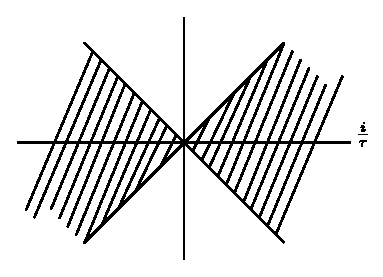
\includegraphics{vol2-figures/fig2.17.eps}}
\end{figure}

Take\pageoriginale $\tau= i t$, $t>0$; then
$$
\frac{C(it)}{i} = \frac{\sum e^{- \pi t n^2}}{\sum e^{-(\pi /t)n^2}}
$$

Both numerator and denominator are positive. So $\frac{C(\tau)}{i}$
lies in the right half. So $|\text{arg} \sqrt{\frac{i}{\tau}} | <
\frac{\pi}{4}$ and $\sqrt{\frac{i}{\tau}}$ denotes the principal
branch. The last equality gives:
$$
\sum^\infty_{n=-\infty} e^{- \pi i n^2/\tau} = \sqrt{\frac{\tau}{i}}
\sum^\infty_{n=-\infty}  e^{\pi i n^2 \tau}
$$

This is a very remarkable formula. It gives a functional relation: the
transformation $\tau \to - 1/\tau$ almost leaves the function
unchanged; it changes only by a simple algebraic function. This is one
of the achievements of Jacobi. 

In the earlier equations we can now put $C(\tau) =
\sqrt{(i/\tau)}$. In particular envisage $\mathscr{V}_1'$:
$$
\displaylines{\hfill \mathscr{V}_1' (0 /\tau) = \left(
  \sqrt{\frac{i}{\tau}}\right)^3 \mathscr{V}_1' \left(0 / -
  \frac{1}{\tau}\right) \hfill \cr
  \text{or} \hfill \mathscr{V}_1' \left(0/-\frac{1}{\tau}\right)=
  \sqrt{\frac{\tau}{i}} \cdot \frac{\tau}{i} \mathscr{V}_1' (o /
  \tau)\hfill}
$$

But 
$$
\displaylines{\hfill \mathscr{V}_1' (0/ \tau) = 2 \pi e^{\pi i \tau/4}
  \prod^\infty_{m=1} (1- e^{2 \pi i m \tau})^3\hfill \cr
  \therefore \hfill e^{- \pi i \tau/4} \prod^\infty_{m=1} (1- e^{- 2
    \pi i m/\tau})^3 = \sqrt{\frac{\tau}{i}} \cdot \frac{\tau}{i}
  e^{\pi i \tau/4} \prod^\infty_{m=1} (1- e^{2 \pi i m \tau})^3 \hfill }
$$

Extracting\pageoriginale cube roots on both sides,
$$
e^{-\pi i \tau/12} \prod^\infty_{m=1} (1- e^{-2 \pi i m/\tau}) = \epsilon
\sqrt{\frac{\tau}{i}} e^{\pi i \tau/12} \prod^\infty_{m=1} (1- e^{2
  \pi i m \tau}) 
$$
where $\epsilon^3 =1$. Dedekind first introduced the function 
$$
\eta (\tau) = e^{\pi i \tau /12} \prod^\infty_{m=1} (1- e^{2 \pi i m \tau})
$$

Then 
$$
\eta\left(- \frac{1}{\tau}\right) = \epsilon\sqrt{\frac{\tau}{i}} \eta (\tau)
$$

This is challenging; we have to decide which $\epsilon$ to take:
$\epsilon^3=1$. The quotient $\eta(-\frac{1}{\tau})\Big/
\sqrt{\frac{\tau}{i}} \eta (\tau)$ is an analytic (hence contains)
function in the upper half-plane and so must be situated in on of the
three open sectors. Now make a special choice; put $\tau=i$. Then
$\eta(i)= \epsilon(+1) \eta (i)$, or $\epsilon=1$.

\medskip
$\therefore$ \hspace{2cm} $\eta \left(- \dfrac{1}{\tau}\right)=
\sqrt{\dfrac{\tau}{i}} \eta (\tau)$
\medskip

What\pageoriginale we have done by considering the lattice of periods can be done in
more sophisticated ways. One can have a whole general theory of the
transformations from 1, $\tau$, to 1, $\dfrac{a \tau+b}{c
  \tau+d}$. The quotients appear first and can be carried over. We
start with $\mathscr{V}_1$ and come back to it; there may be
difficulty, however in deciding the sign. 
